\documentclass[11pt]{article}
\usepackage[margin=0.9in]{geometry}
\usepackage{amsmath,amssymb}
\usepackage{booktabs}
\usepackage[table]{xcolor}
\usepackage{pgfplots}
\pgfplotsset{compat=1.18}
\usepackage{tikz}
\usepackage{caption}
\usepackage[colorlinks=true,linkcolor=blue,urlcolor=blue,citecolor=blue]{hyperref}
\usepackage{enumitem}
\setlist{nosep,leftmargin=1.4em}
\usepackage{titlesec}
\titlespacing*{\section}{0pt}{1.1ex}{0.6ex}
\titlespacing*{\subsection}{0pt}{0.8ex}{0.4ex}
\setlength{\parskip}{0.4ex}
\setlength{\parindent}{0pt}

\definecolor{good}{RGB}{27,158,119}
\definecolor{mid}{RGB}{217,95,2}
\definecolor{scale}{RGB}{31,120,180}
\definecolor{bad}{RGB}{192,57,43}
\definecolor{blu}{RGB}{44,111,187}
\definecolor{gry}{RGB}{136,136,136}
\definecolor{hl}{RGB}{240,240,240}

\title{\vspace{-3em}\textbf{Cascade direction from a single-cell snapshot:\\
the method, the coupling fix, and where direction reverses}}
\author{\normalsize cytokine-MIL project --- consolidated progress report}
\date{\vspace{-1em}\normalsize 2026-06-25}

\begin{document}
\maketitle
\vspace{-2.0em}

\begin{abstract}
\noindent\textbf{How it works:} from one snapshot of perturbed immune cells we give each
condition a \emph{discovered} gene signature, then read how much each condition's cells express
\emph{another} condition's signature --- the symmetric part of that cross-engagement tells us
\emph{whether} two conditions are coupled, the antisymmetric part (\texttt{cross\_asym}) tells us
\emph{who is upstream}. \textbf{What it can do:} recover known cytokine cascades and their
direction across five datasets ($83$--$88\%$ directional accuracy) and recover a disease/
vaccination \emph{progression} timeline from a cross-section. \textbf{The gate fix:} the
coupling-existence test used to over-call ($\sim$77\% of pairs ``coupled''); a donor-level null
plus a hub/degree correction nearly halved the over-call (to 31\%) \emph{while raising} known-pair
recall ($8/17\!\to\!11/17$), and is symmetric so it never touches the direction call.
\textbf{The reverse finding:} on a T-cell \emph{differentiation} axis the direction call comes out
\emph{exactly backwards} --- because \texttt{cross\_asym} assumes the upstream cell \emph{acquires}
the downstream program, whereas differentiation is the opposite (the mature cell \emph{retains}
the progenitor's program); a synthetic ``tree'' control reproduces the reversal and pins it on the
acquisition-vs-retention asymmetry, not on topology.
\end{abstract}

\section{The method, exactly (and short)}
We never label cells by hand. For every condition $X$ (a cytokine, a stimulus, a state, a
time-point) we train a small attention-MIL model to tell ``$X$ vs.\ control'' and read out its
\textbf{discovered signature} $S_X$ = the top-50 genes by Integrated Gradients through the model.
Direction and coupling then both come from one quantity --- how much condition $a$'s cells express
condition $b$'s signature, PBS/control-normalised, computed \emph{per cell type} and then
aggregated (median across cell types):
\begin{equation}
M[a,b]\;=\;s(a,S_b)\;-\;s(\mathrm{control},S_b),
\qquad s(x,S)=\text{mean expression of gene set }S\text{ in population }x .
\end{equation}
The matrix $M$ splits into a symmetric and an antisymmetric half, and \emph{that split is the
whole method}:
\begin{equation}
\underbrace{\text{coupling}(a,b)=M[a,b]+M[b,a]}_{\text{symmetric}\;\Rightarrow\;\text{do they engage each other? (existence)}}
\qquad
\underbrace{\mathrm{cross\_asym}(a,b)=M[a,b]-M[b,a]}_{\text{antisymmetric}\;\Rightarrow\;\text{who is upstream? (direction)}}
\end{equation}
Spelled out with the control term, the direction statistic is
\begin{equation}
\mathrm{cross\_asym}(a,b)=\underbrace{\big[s(a,S_b)-s(b,S_a)\big]}_{\text{raw cross-engagement}}
-\underbrace{\big[\mathrm{ctrl}_{S_b}-\mathrm{ctrl}_{S_a}\big]}_{\text{control term}} .
\label{eq:cross}
\end{equation}
\textbf{The biology it encodes:} an \emph{upstream} stimulus's cells carry \emph{both} their own
and the (autocrine) \emph{downstream} program, so $s(\text{up},S_{\text{down}})>s(\text{down},
S_{\text{up}})$ and $\mathrm{cross\_asym}$ is positive in the upstream-first direction. It is
antisymmetric by construction ($\mathrm{cross\_asym}(b,a)=-\mathrm{cross\_asym}(a,b)$), so its
\emph{sign} encodes the arrow. Direction is read \emph{only} on pairs the coupling gate already
calls coupled --- existence and direction are two different questions.

\section{The coupling-gate fix}
The gate decides ``are $a,b$ coupled?''. The old version \textbf{over-called} ($\sim$77\% of
Oesinghaus pairs ``coupled'') for two reasons:
\begin{itemize}
\item \textbf{Over-power.} The significance null was computed at the \emph{cell} level (thousands
of cells), so every mean was razor-sharp and almost everything beat the null. The true unit of
independence is the \emph{donor} ($\sim$10), not the cell.
\item \textbf{Hub/degree bias.} A broadly-engaged signature (e.g.\ IL-15, induced by many
cytokines) looks coupled to \emph{everything}; this lives in the coupling value itself and
survives even a perfect null.
\end{itemize}
\textbf{The fix.} Replace the cell null with a \textbf{donor-level sign-flip null} (unit $=$
donor), and remove hubs by \textbf{degree double-centering} of the coupling matrix,
$R[i,j]=C[i,j]-d_i-d_j+g$ ($d_i$ = node strength, $g$ = grand mean). The degree correction is
symmetric, so it \emph{only} sharpens existence and \textbf{never alters direction}. Degree
correction was the decisive piece; specificity-only fixes (panel-residualised signatures) did
\emph{not} reduce over-call.

\begin{table}[h]\centering\small
\caption*{\textbf{Table 1.} Coupling gate on Oesinghaus, fix applied step by step.}
\begin{tabular}{lccc}
\toprule
Gate variant & null unit & over-call & known-pair recall \\
\midrule
old (cell-level null) & cells ($\sim10^3$) & $\sim$77\% & 8/17 \\
\ + donor-level null & donors ($\sim$10) & 53\% & 8/17 \\
\rowcolor{hl}\ + degree correction & donors & \textbf{31\%} & \textbf{11/17} ($2.1\times$) \\
\bottomrule
\end{tabular}
\end{table}

\textbf{Does the trained encoder earn its place?} Yes. Holding everything else fixed and swapping
\emph{only} how $S_X$ is defined (Integrated Gradients \emph{through the model} vs.\ plain
differential expression, $\times$ two contrasts), DE collapses direction to chance and selects
near-disjoint genes (Jaccard$=0.11$ with IG). The model's attributions carry signal a fold-change
list does not.

\begin{table}[h]\centering\small
\caption*{\textbf{Table 2.} Signature ablation on Oesinghaus --- the encoder is not removable.}
\begin{tabular}{lccc}
\toprule
signature & direction acc.\ & coupled frac.\ & top hub \\
\midrule
\rowcolor{hl}IG, vs-PBS (current) & \textbf{14/17 (82\%)} & 76.5\% & IL-15 \\
IG, vs-Panel & 14/17 (82\%) & 77.9\% & IL-15 \\
DE, vs-PBS & 10/17 (59\%) & 58.7\% & IFN-$\beta$ \\
DE, vs-Panel & 9/17 (53\%) & 46.7\% & IFN-$\beta$ \\
\bottomrule
\end{tabular}
\end{table}

\section{What it can and can't do --- across five datasets}
All numbers use the \textbf{updated method} (signature coupling $+$ donor/degree fix $+$
\texttt{cross\_asym} direction). Three dataset levers --- number of perturbation labels, number of
donors, and whether the labels stand in a directional relationship --- determine where the method
works.

\begin{table}[h]\centering\small
\caption*{\textbf{Table 3.} Dataset metadata (the levers).}
\begin{tabular}{llrrrll}
\toprule
dataset & organism / tissue & cells & donors & cell types & labels & panel \\
\midrule
Oesinghaus & human PBMC, 24h & $\sim$9.7M & 12 & $\sim$18 & 90 cyt & whole-tx \\
Sheu & mouse BMDM, 3h & $\sim$295K & 4$^\ast$ & $\sim$3 & 7 stim & \textbf{500-gene} \\
Imm.\ Dict.\ (Cui) & mouse LN, \emph{in vivo} 4h & $\sim$387K & 3/cyt & 26 & 86 cyt & whole-tx \\
Cano-Gamez & human CD4 T & 43K & 4 & 2 & 4 Th & whole-tx \\
Oelen & human PBMC & $\sim$911K & \textbf{128} & 9 & 6 path$\times$t & whole-tx \\
\bottomrule
\end{tabular}
\end{table}
\vspace{-0.7em}
{\footnotesize $^\ast$pseudo-donors. Whole-tx datasets reduced to 4000 HVG; coupling used a
binary-IG label subset where training cost required it (Oes 24, Cui 12).}

\begin{table}[h]\centering\small
\caption*{\textbf{Table 4.} Results with the updated method.}
\begin{tabular}{lllll}
\toprule
dataset & coupling over-call & coupling recall & direction (cross\_asym) & gate path \\
\midrule
Oesinghaus & $77\to\textbf{31}\%$ & \textbf{11/17} ($2.1\times$) & \textbf{88\%} (15/17) & donor+degree \\
Sheu & $\to$43\% & 4/5 MUST$^\dagger$ & \textbf{86\%} (6/7) & cell+degree \\
Imm.\ Dict. & $88\to\textbf{44}\%$ & \textbf{6/7} & \textbf{83\%} (5/6) & cell+degree \\
Cano-Gamez & $100\to\textbf{33}\%$ & Th17$\leftrightarrow$iTreg \#1 & n/a (parallel fates) & cell+degree \\
Oelen & $33\to47\%^\ddagger$ & 1/3 & progression 2/3 & donor @128 \\
\bottomrule
\end{tabular}
\end{table}
\vspace{-0.7em}
{\footnotesize $^\dagger$latent-geometry coupling \emph{failed} 0/2 on Sheu's targeted panel;
signature-space coupling \emph{rescued} 2/2 IFN cascades. $^\ddagger$too few labels (6) for degree
correction to help.}

\begin{figure}[h]\centering
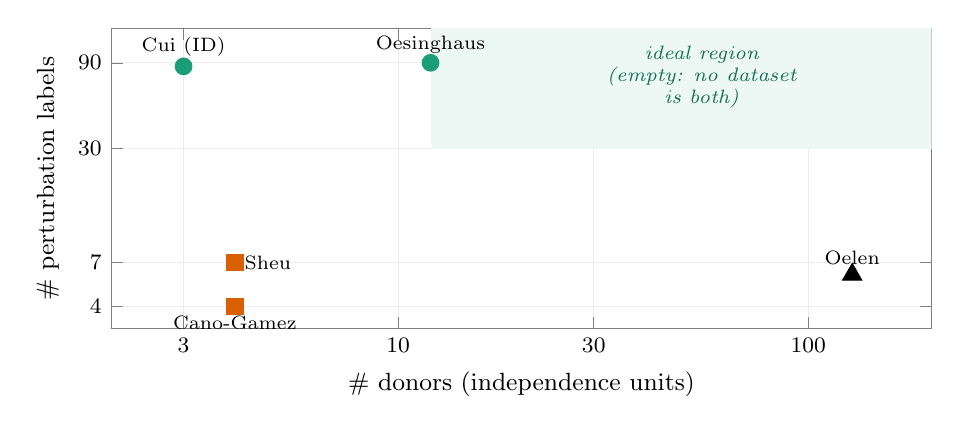
\begin{tikzpicture}
\begin{axis}[
  width=12.0cm, height=5.4cm,
  xmode=log, ymode=log, log basis x=10, log basis y=10,
  xlabel={\# donors (independence units)}, ylabel={\# perturbation labels},
  xmin=2, xmax=200, ymin=3, ymax=140,
  xtick={3,10,30,100}, xticklabels={3,10,30,100},
  ytick={4,7,30,90}, yticklabels={4,7,30,90},
  tick label style={font=\footnotesize}, label style={font=\small},
  axis line style={draw=gray}, grid=both, grid style={gray!15},
]
\fill[good!8] (axis cs:12,30) rectangle (axis cs:200,140);
\node[good!70!black,font=\scriptsize\itshape,align=center] at (axis cs:55,75)
  {ideal region\\(empty: no dataset\\is both)};
\addplot[only marks,mark=*,good,mark size=3pt] coordinates {(12,90) (3,86)};
\addplot[only marks,mark=square*,mid,mark size=3pt] coordinates {(4,7) (4,4)};
\addplot[only marks,mark=triangle*,scale,mark size=4pt] coordinates {(128,6)};
\node[anchor=south,font=\scriptsize] at (axis cs:12,90) {Oesinghaus};
\node[anchor=south,font=\scriptsize] at (axis cs:3,86) {Cui (ID)};
\node[anchor=west,font=\scriptsize] at (axis cs:4,7) {Sheu};
\node[anchor=north,font=\scriptsize] at (axis cs:4,4) {Cano-Gamez};
\node[anchor=south,font=\scriptsize] at (axis cs:128,6) {Oelen};
\end{axis}
\end{tikzpicture}
\caption*{\textbf{Figure 1.} The method needs \emph{both} many donors (powered null) \emph{and}
many labels (stable degree correction). \textcolor{good}{Green}: coupling+direction work;
\textcolor{mid}{orange}: partial; \textcolor{scale}{blue}: donor-scale milestone but too few
labels. The joint ``ideal'' corner is empty --- the standing gap.}
\end{figure}

\textbf{Four metadata-driven rules.}
\textbf{(1)} \emph{\# labels governs degree correction} --- works at $\gtrsim$15--20 conditions
(Oes, Cui), fails at 4--6 (Cano, Oelen). \textbf{(2)} \emph{\# donors governs the gate path} ---
$<$8 donors $\Rightarrow$ cell-level fallback; $\geq$8 $\Rightarrow$ powered donor-level null
(Oelen's 128 is the scale proof). \textbf{(3)} \emph{Panel breadth governs the shared-activation
confound} --- a targeted 500-gene panel (Sheu) collapses latent geometry, but signature space
(specific genes) is panel-robust. \textbf{(4)} \emph{Label semantics govern whether direction
exists} --- cytokine perturbations with known cascades give direction (83--88\%); parallel fates
(Cano) or pathogens (Oelen) give coupling/progression only. \emph{Net:} Oesinghaus uniquely has
all three (many labels $+$ $\geq$8 donors $+$ directional perturbations); every other dataset is
missing one, exactly where it underperforms.

\section{The reverse finding: a recovered timeline but an inverted state order}
We pushed the direction statistic onto a \textbf{T-cell maturation} axis
(naive$\rightarrow$effector$\rightarrow$memory) on a public SARS-CoV-2 vaccination whole-PBMC
CITE-seq atlas (\emph{Nat.\ Immunol.}\ 2023; days 0/2/11/28, 6 donors, 61{,}911 T cells), reusing
the disease-progression pipeline verbatim under two framings. \textbf{STATE:} condition $=$
\{Naive, Effector, Memory\} read from CITE \emph{surface protein} (CD45RO/CD27 --- RNA-independent,
so state labels cannot leak into the RNA signatures), control $=$ day-0 ``Resting''.
\textbf{TIMEPOINT:} condition $=$ \{D2, D11, D28\}, control $=$ D0. An independent synthetic
\emph{apparatus} supplies a distinct-program go/no-go gate.

\begin{table}[h]\centering\small
\caption*{\textbf{Table 5.} Direction recovery: the apparatus passes, the timeline is recovered,
the state order is exactly inverted.}
\begin{tabular}{lcccl}
\toprule
framing & \texttt{cross\_asym} acc.\ & symm.\ control & Kendall $\tau$ & verdict \\
\midrule
Apparatus (distinct-program gate) & $100\%$ & $50\%$ & $+1.0$ & \textcolor{good}{PASS} \\
\textbf{Timepoint} D2$<$D11$<$D28 & $\mathbf{100\%}$ & $0\%$ & $\mathbf{+1.0}$ & \textcolor{mid}{AMBER}$^\dagger$ \\
\textbf{State} Naive$<$Eff$<$Mem & $\mathbf{0\%}$ & $100\%$ & $\mathbf{-1.0}$ & \textcolor{bad}{RED (reversed)} \\
\bottomrule
\end{tabular}
\end{table}
\vspace{-0.7em}
{\footnotesize $^\dagger$Timepoint is AMBER \emph{only} because the 6-donor bootstrap CI is wide
($[0.33,1.0]$); the point estimate is perfect. Recovered orders: timepoint $=$
D2$\rightarrow$D11$\rightarrow$D28 (truth); state $=$ Memory$\rightarrow$Effector$\rightarrow$Naive
(the exact reverse of truth, hence $\tau=-1.0$).}

The tell-tale is the relationship between the direction statistic and its \emph{symmetric} control
(\texttt{directional\_score}). On the apparatus and timepoint axes \texttt{cross\_asym} $\gg$
control (the healthy cytokine/COVID pattern); on the state axis the two \emph{swap}
(Fig.~\ref{fig:bars}) --- the synthetic ``no-seed'' regime, reproduced in real data (Fig.~2).

\begin{figure}[h]
\centering
\scalebox{0.82}{%
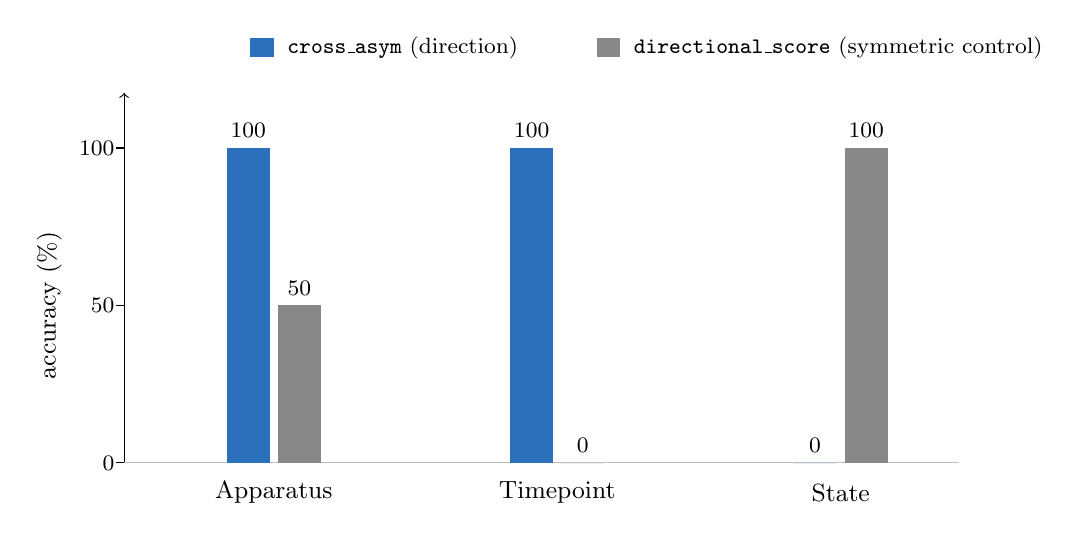
\begin{tikzpicture}
\draw[->] (0,0) -- (0,4.7);
\node[rotate=90,font=\small] at (-0.95,2.0) {accuracy (\%)};
\foreach \p/\y in {0/0, 50/2.0, 100/4.0} {\draw (-0.1,\y)--(0,\y) node[left,font=\footnotesize]{\p};}
\draw[gray!50] (0,0) -- (10.6,0);
\fill[blu] (1.30,0) rectangle (1.85,4.00); \node[font=\footnotesize] at (1.575,4.22){100};
\fill[gry] (1.95,0) rectangle (2.50,2.00); \node[font=\footnotesize] at (2.225,2.22){50};
\node[font=\small] at (1.90,-0.38){Apparatus};
\fill[blu] (4.90,0) rectangle (5.45,4.00); \node[font=\footnotesize] at (5.175,4.22){100};
\fill[gry] (5.55,0) rectangle (6.10,0.00); \node[font=\footnotesize] at (5.825,0.22){0};
\node[font=\small] at (5.50,-0.38){Timepoint};
\fill[blu] (8.50,0) rectangle (9.05,0.00); \node[font=\footnotesize] at (8.775,0.22){0};
\fill[gry] (9.15,0) rectangle (9.70,4.00); \node[font=\footnotesize] at (9.425,4.22){100};
\node[font=\small] at (9.10,-0.38){State};
\fill[blu] (1.6,5.15) rectangle (1.9,5.4); \node[right,font=\footnotesize] at (1.95,5.27){\texttt{cross\_asym} (direction)};
\fill[gry] (6.0,5.15) rectangle (6.3,5.4); \node[right,font=\footnotesize] at (6.35,5.27){\texttt{directional\_score} (symmetric control)};
\end{tikzpicture}}
\caption*{\textbf{Figure 2.} The ``inverse fingerprint.'' On the apparatus and timepoint axes the
antisymmetric direction statistic beats its symmetric control; on the state axis the two swap
places --- direction $0\%$, control $100\%$ --- the hallmark of an axis where \texttt{cross\_asym}'s
core assumption runs backwards.}
\end{figure}

\textbf{We falsified our own first explanation.} The obvious guess was ``the day-0 control
$\approx$ Naive, so the upstream state coincided with the baseline.'' A \emph{control-swap
decomposition} (holding the signatures fixed, varying only the control term in
Eq.~\eqref{eq:cross}, including a \texttt{ZERO} control $=$ pure cross-engagement) refutes it:
the \emph{raw} engagement is the \emph{most} inverted ($+0.588$ vs $+0.140$ under Resting), the
control \emph{reduces} the inversion, and \emph{no} control choice un-inverts the Naive pairs
($\tau=-1.0$ throughout). The inversion is intrinsic to the axis.

\begin{table}[h]\centering\small
\caption*{\textbf{Table 6.} Control-swap decomposition --- the reversal is control-independent.
Correct sign for an $X$--Naive pair is \emph{negative} (Naive upstream); every control gives
\emph{positive}.}
\begin{tabular}{lccc}
\toprule
control & \texttt{cross\_asym}(Eff,Nai) & \texttt{cross\_asym}(Mem,Nai) & $\tau$ \\
\midrule
Resting (original)                      & $+0.107$ & $+0.140$ & $-1.0$ \\
\rowcolor{hl}\textbf{ZERO} $=$ raw engagement & $\mathbf{+0.253}$ & $\mathbf{+0.588}$ & $-1.0$ \\
Balanced (removes naive/mem imbalance)  & $+0.121$ & $+0.146$ & $-1.0$ \\
Naive as control                        & $+0.138$ & $+0.147$ & $-1.0$ \\
Memory as control                       & $+0.159$ & $+0.161$ & $-1.0$ \\
\bottomrule
\end{tabular}
\end{table}

\textbf{The mechanism.} \texttt{cross\_asym} assumes program \emph{acquisition}: the upstream cell
\emph{gains} the downstream program (cytokine-autocrine logic). Differentiation is the opposite ---
a program-\emph{retention} asymmetry: the \emph{mature} cell \emph{retains} the \emph{progenitor's}
program (memory T cells re-express the naive program \textit{IL7R, TCF7, SELL, CCR7}). Hence
$s(\text{Memory},S_{\text{Naive}})\gg s(\text{Naive},S_{\text{Memory}})$ and the statistic
faithfully points mature$\rightarrow$naive. This is not a bug (the apparatus distinct-gate passes)
and not fixable by control choice; it is the method meeting an axis whose biology is sign-flipped
relative to its assumption.

\subsection{A synthetic ``tree'' confirms: it is acquisition-vs-retention, not topology}
To rule out ``maybe the chain just has to be linear,'' we built a 4th synthetic scenario
(\emph{new this session}): a partial-order \textbf{tree} $p_0\!\to\!p_1,\,p_1\!\to\!p_2,\,
p_0\!\to\!p_3$ where each node carries its own program block \emph{plus half its parent's full
program} (a pure \emph{retention} structure --- the descendant carries the ancestor), with
\emph{identical} hyperparameters to the three ladder scenarios so the four are directly
comparable. The tree reproduces the no-seed/retention regime exactly: \texttt{cross\_asym}
mis-signs \emph{all four} ancestor$\to$descendant edges (each names the descendant as upstream),
while the two incomparable sibling pairs stay correctly $\approx$ambiguous; the reversal magnitude
even tracks the carried fraction (direct edges $|\mathrm{cross\_asym}|\!\approx\!0.61$; the
transitive grandparent edge $\approx\!0.26$).

\begin{table}[h]\centering\small
\caption*{\textbf{Table 7.} Four comparable synthetic scenarios (same hyperparameters). A
retention structure inverts \texttt{cross\_asym} whether the topology is a chain or a tree;
a distinct-program (acquisition-style) structure is recovered perfectly.}
\begin{tabular}{lccc}
\toprule
scenario & \texttt{cross\_asym} acc.\ & symm.\ control & Kendall $\tau$ \\
\midrule
\rowcolor{hl}distinct (acquisition / seeded) & \textbf{100\%} & 50\% & $+1.00$ \\
monotone\_noseed (retention) & 0\% & 50\% & $-1.00$ \\
monotone\_seeded (mixed) & 67\% & 50\% & $+0.33$ \\
\rowcolor{hl}\textbf{tree} (retention, non-linear) & \textbf{0\%} & 50\% & $\mathbf{-1.00}$ \\
\bottomrule
\end{tabular}
\end{table}

\section{Synthesis: an identifiability problem, and how to break it}
The reversal is not a defect of the statistic --- it is a genuine \textbf{identifiability problem}.
A single observation $\mathrm{cross\_asym}(X,Y)>0$ (``$X$'s cells carry more of $Y$'s program than
vice versa'') is consistent with \emph{two opposite truths}: \textbf{(i)} $X$ is upstream and is
\emph{inducing} $Y$'s program (acquisition --- cytokine/timeline case, sign correct), or
\textbf{(ii)} $Y$ is upstream and $X$ is \emph{derived from} $Y$ and retains its residual program
(retention --- differentiation case, sign reversed). The snapshot alone cannot tell these apart.
This separates cleanly into how the method should be \emph{used}:
\begin{itemize}
\item $|\mathrm{cross\_asym}|$ (and $\text{coupling}=M+M^{\top}$) $=$ \textbf{coupling strength}:
robust and regime-independent. The tree confirms it --- it fired confidently on every real edge
and correctly abstained ($\approx0$) on unrelated siblings.
\item $\mathrm{sign}(\mathrm{cross\_asym})$ $=$ \textbf{direction}: interpretable only once the
\emph{regime} (acquisition vs.\ retention) is fixed. Confidently right under acquisition,
confidently \emph{wrong} under retention.
\end{itemize}
Fixing the regime needs an \textbf{arrow from outside the snapshot} --- exactly the classic
trajectory-inference identifiability issue (why RNA velocity needs a spliced/unspliced clock). The
practical disambiguators: \textbf{(a) time or a perturbation} sets the arrow directly --- which is
\emph{why the timepoint framing worked and the state framing did not} (the vaccine imposes
$t_0$; a pure cross-section of one lineage has no arrow); \textbf{(b) a known root / applied
stimulus} (the cytokine case --- the perturbation \emph{is} the upstream); \textbf{(c) lineage
constraints} (two different cell types cannot be related by differentiation, so a shared signature
there is more likely acquisition); \textbf{(d) the gene-class of the carried program} ---
induction tends to leave the downstream's \emph{inducible/response} genes in the upstream, whereas
retention leaves the upstream's \emph{identity/TF} genes in the downstream, a potential
\emph{internal} discriminator we have not yet tested.

\textbf{Bottom line for the project.} The coupling gate is fixed and validated; the direction
statistic is validated on acquisition-type axes (cytokine cascades $83$--$88\%$; vaccination/
disease progression timelines). We have now \emph{mapped its boundary}: on cell-state
differentiation axes it is a faithful \emph{coupling} detector but a sign-flipped \emph{direction}
detector, and we understand precisely why. The next milestones follow directly: an
acquisition-vs-retention discriminator (the gene-class probe, or a forward-seed/backward-carry
synthetic pair), a donor-level \emph{direction} null for novel-pair claims, and a dataset that is
simultaneously high-donor \emph{and} many-label \emph{and} directional --- the empty ``ideal''
corner of Figure~1.

\end{document}
